\section{Long Horizon Risk: Analytical vs. Simulation}
\textbf{Question 1.1}: Consider that if the DGP accurate then the volatility is time-varying 
and dependent on both returns $R_t$ and $\sigma_t$ as shown in the formula:
$$\sigma_{t+1}^2=\omega+\alpha R_t^2+\beta \sigma_t^2$$
Then intuitively the analytical \textbf{model 1} is misspecified because 
assuming that the K-day cumulative 
return distribution is distributed as $N(0,K\sigma_{t+1}^2)$ fails to account for 
time-varying volatility during each subsequent day and instead erroneously assumes
constant volatility that simply needs to be scaled by the number of days $K$. \\ \\
Alternatively, simulation \textbf{model 2} is \textit{not} misspecified because each
day generates a shock $\check{z} \sim N(0,1)$ and updates
the variance using:
$$\check{\sigma_{t+1}^2}=\omega+\alpha \check{R_t^2}+\beta \check{\sigma_t^2}$$
which incorporates path dependency on the previous day's shocks and volatilities, 
therefore allowing for time-varying volatility to be captured on a day-to-day basis. 
\\ \\ 
\textbf{Question 1.2}: The estimated GARCH(1,1) for Apple's stock data was modeled 
using the python library \texttt{arch} with the function \texttt{archmodel} with
a statistifically significant p-value:
$$\sigma_{t+1}^2=0.000009+(0.1) R_t^2+(0.88) \sigma_t^2$$

Using the GARCH(1,1) model estimated above, both models were implemented according
to the methods described in lecture notes to model and graph the 
$\text{VaR}_{t+K}^{1\%}$ based on K-day cummulative returns.

\begin{figure}[H]
    \centering 
    \begin{minipage}{.47\textwidth}
        \centering
        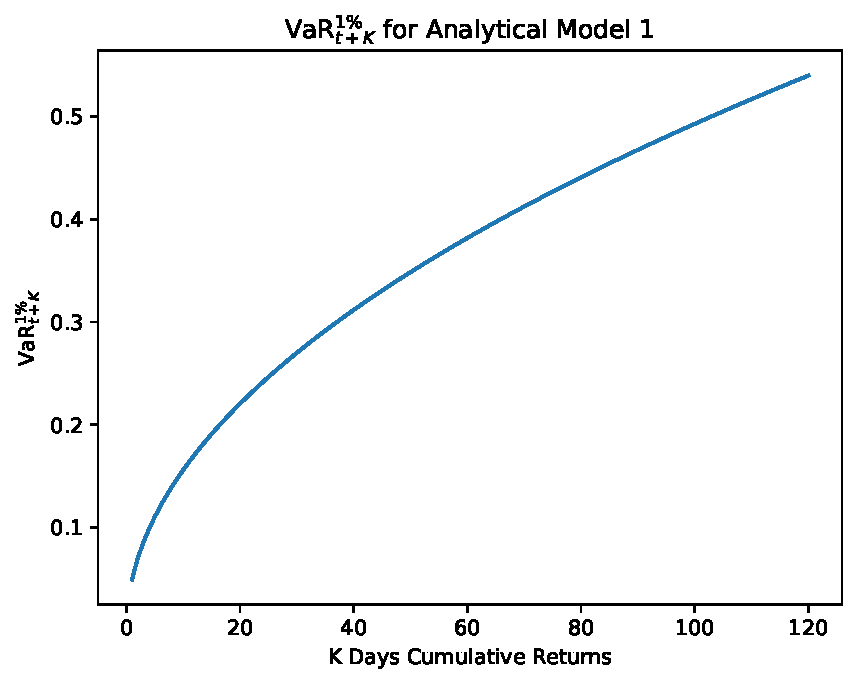
\includegraphics[width=\textwidth]{./figures/ECO491_HW4_Q1_Model_1.pdf}
        \caption{Analytical Model 1}
        \label{fig:model1}
    \end{minipage}
    \hfill
    \begin{minipage}{.47\textwidth}
        \centering
        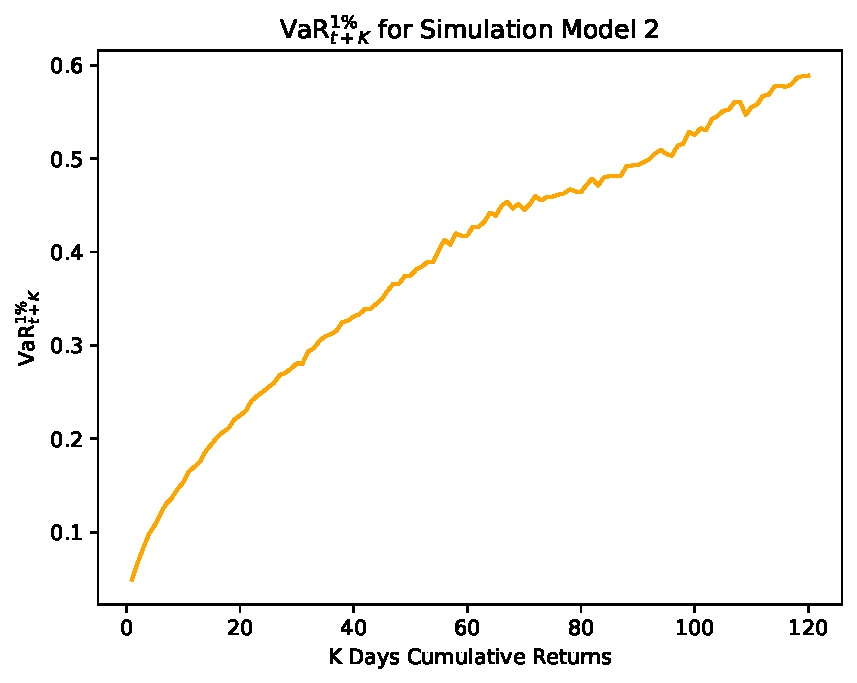
\includegraphics[width=\textwidth]{./figures/ECO491_HW4_Q1_Model_2.pdf}
        \caption{Simulation Model 2}
        \label{fig:model2}
    \end{minipage}
\end{figure}

The analytical VaR scales with sqrt(K) because it assumes constant volatility. Under GARCH, volatility
persistence causes cumulative variance to grow faster, producing larger tail risk. Therefore Model 2 yields a
higher long-horizon VaR

\textbf{Question 1.3}: The distribution $N(0, K \sigma_{t+1}^2)$ was plotted and
then the values of 10000 different simulated K-day cumulative returns at K = 20 were
superimposed.

\begin{figure}[H]
  \centering
  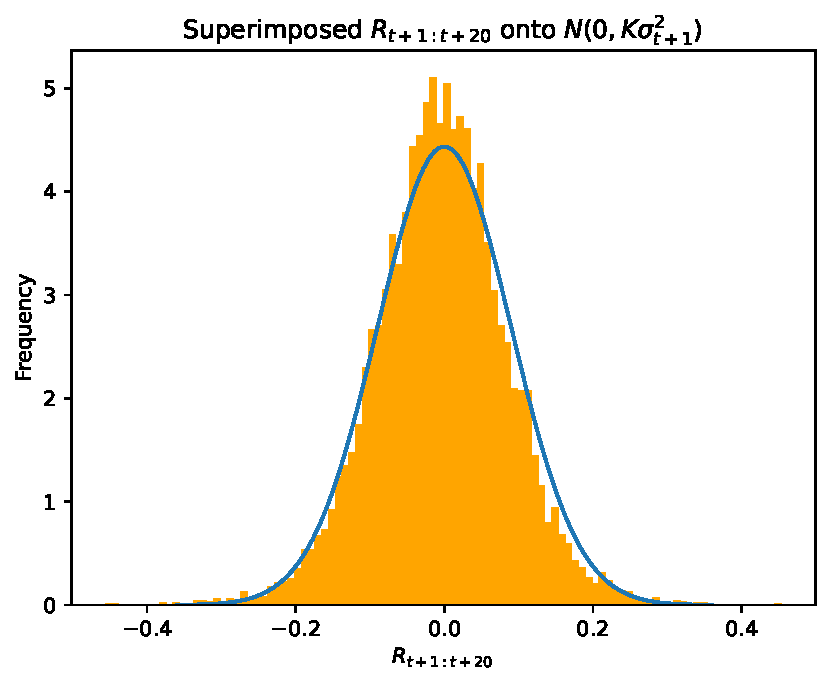
\includegraphics[width=.5\textwidth]{./figures/ECO491_HW4_Q1_Superimpose.pdf}
  \caption{Superimpose $R_{t+1:t+20} \text{ on } N(0, K \sigma_{t+1}^2)$}
\end{figure}

The simulated 20-day return distribution shows skewness and excess kurtosis due to volatility clustering. Early
shocks propagate through the GARCH recursion, generating heavy tails. Thus Model 1 underestimates true VaR.

\section{Interest Rates Risk}

\textbf{Question 2.1}: A model for the term structure of interest rates is not
necessary because the maturity of the zero-coupon bond is the same as the maturity
of the provided fixed maturities.

\begin{figure}[H]
  \centering
  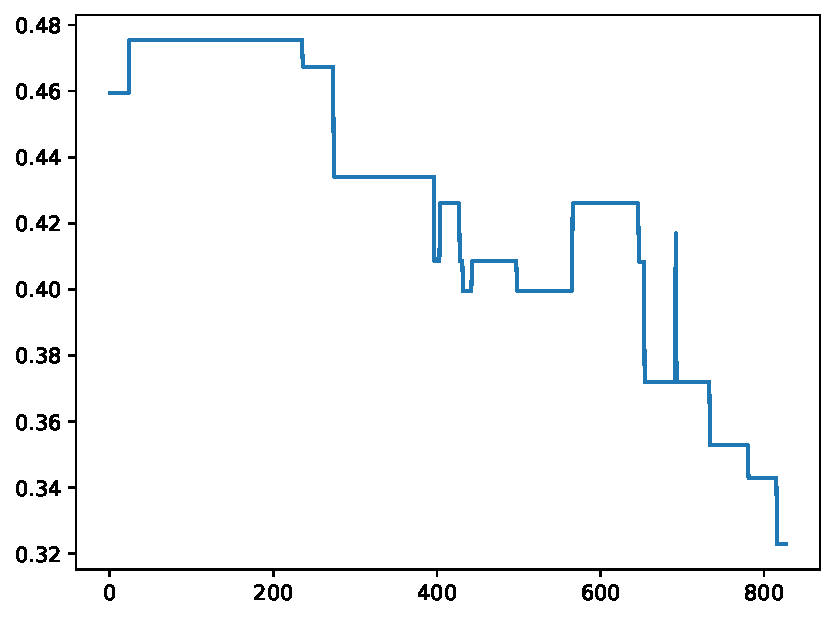
\includegraphics[width=.5\textwidth]{./figures/ECO491_HW4_Q2.1_HS.pdf}
  \caption{Historical Simulation VaR Bond}
\end{figure}

A term structure model is unnecessary because the 3-year yield is directly observed. Historical Simulation
requires only the time series of prices computed using the directly available 3-year yield. A model is needed only
when the bond maturity is not quoted. 

Additionally, the VaR obtained using the polynomial term structure model differs from the direct
historical simulation of Question~2.1 for three reasons:

\begin{enumerate}
\item The polynomial model introduces \emph{curve-fitting error};
      the fitted 3-year yield differs from the observed yield.
\item Historical shocks are applied to the four $\beta$ factors rather than
      directly to the 3-year rate, producing different yield dynamics.
\item The required pricing formula uses
$$
\Delta P = P(t+1,T-\tfrac{1}{252}) - P(t,T)e^{R(t,T)/252},
$$
which incorporates both the maturity roll-down and the carry adjustment.
\end{enumerate}

These differences typically result in a larger and more volatile VaR in 2.2.


\textbf{Question 2.2}: The following graphs are all the time series of all the factor loadings:
\begin{figure}[H]
    \centering 
    \begin{minipage}{.48\textwidth}
        \centering
        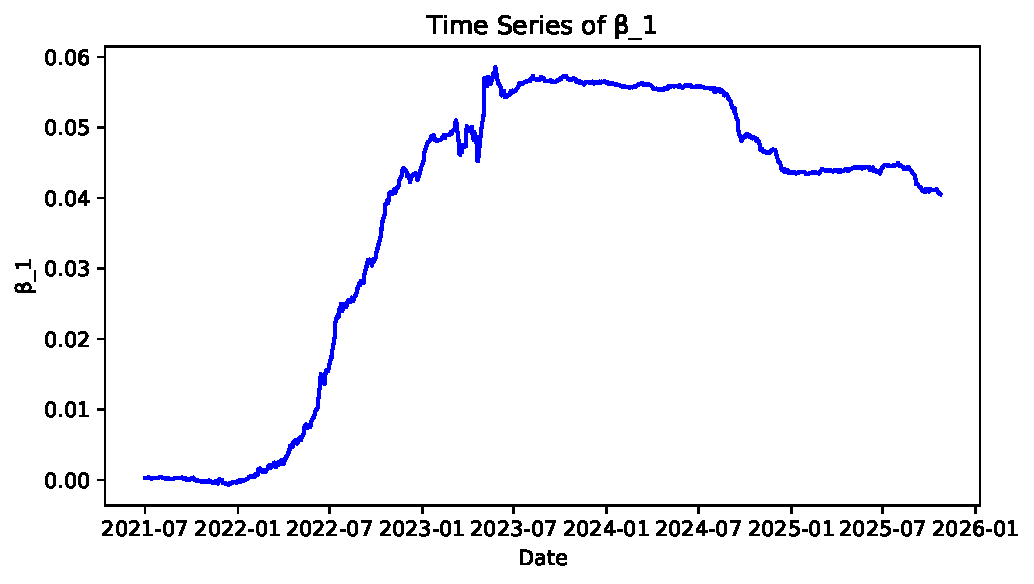
\includegraphics[width=\textwidth]{./figures/ECO491_HW4_Q2.2_β1.pdf}
        \caption{Time Series of $\beta_{1}$}
        \label{fig:model1}
    \end{minipage}
    \hfill
    \begin{minipage}{.48\textwidth}
        \centering
        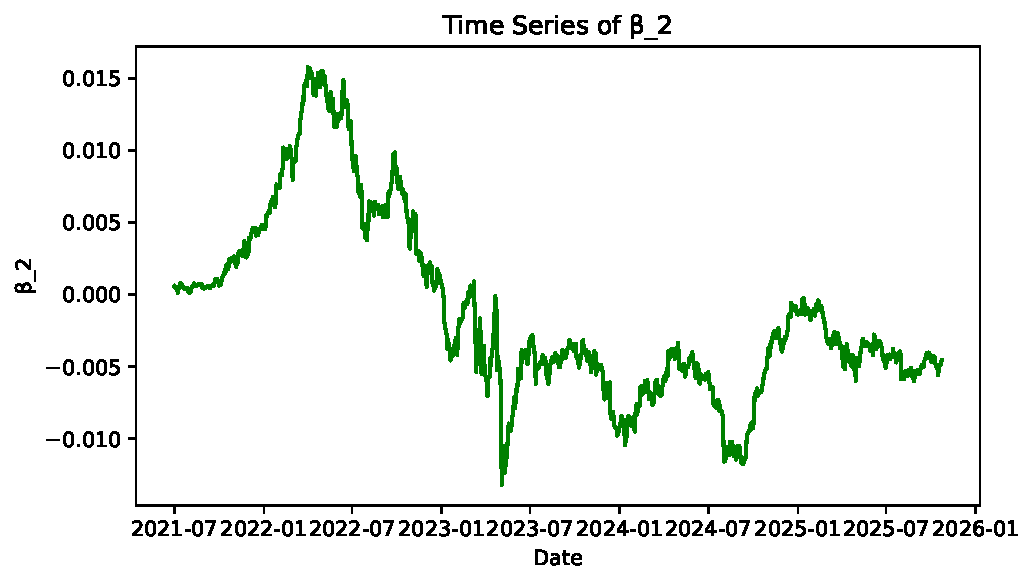
\includegraphics[width=\textwidth]{./figures/ECO491_HW4_Q2.2_β2.pdf}
        \caption{Time Series of $\beta_{2}$}
        \label{fig:model2}
    \end{minipage}
\end{figure}
\begin{figure}[H]
    \centering 
    \begin{minipage}{.48\textwidth}
        \centering
        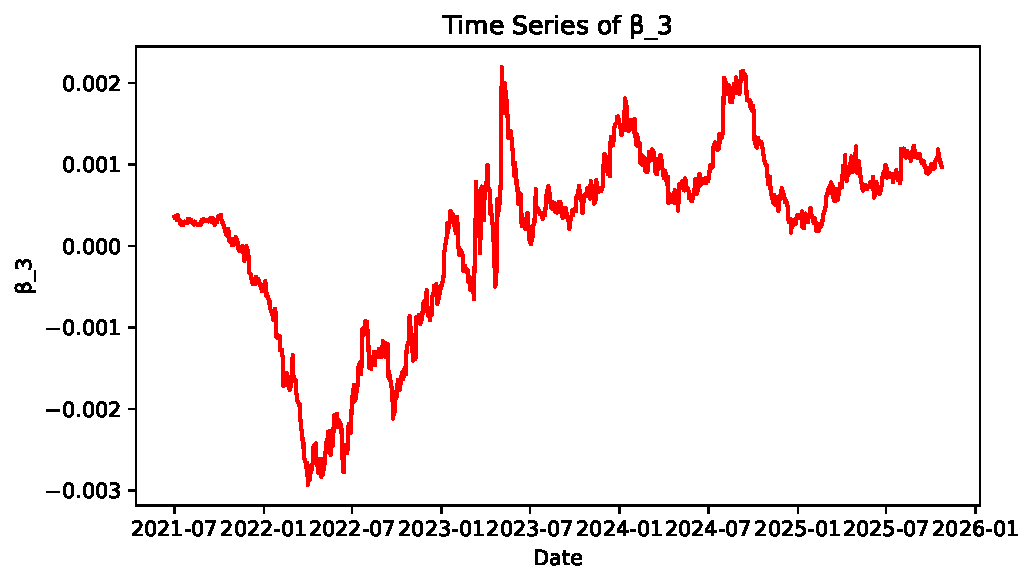
\includegraphics[width=\textwidth]{./figures/ECO491_HW4_Q2.2_β3.pdf}
        \caption{Time Series of $\beta_{3}$}
        \label{fig:model1}
    \end{minipage}
    \hfill
    \begin{minipage}{.48\textwidth}
        \centering
        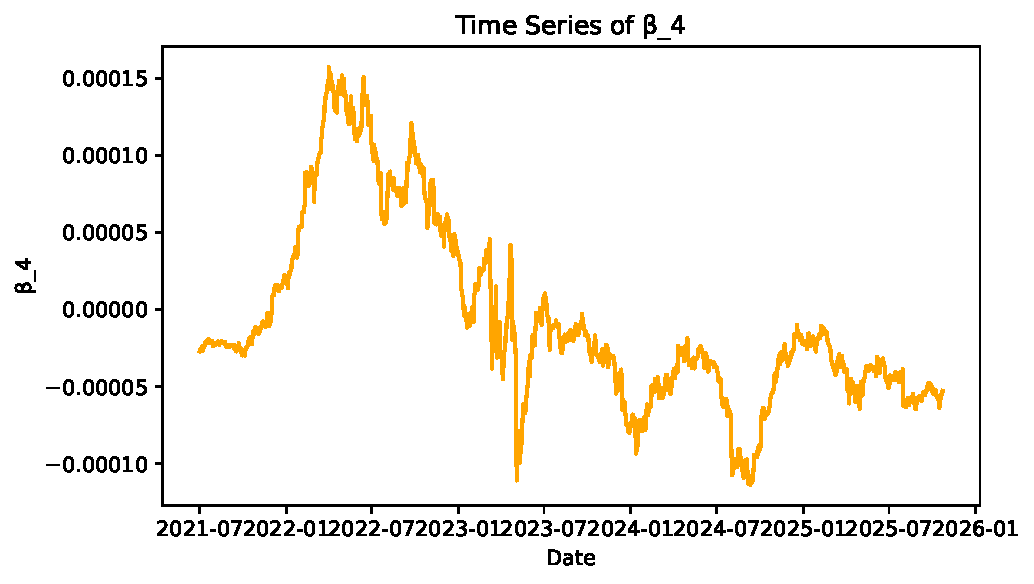
\includegraphics[width=\textwidth]{./figures/ECO491_HW4_Q2.2_β4.pdf}
        \caption{Time Series of $\beta_{4}$}
        \label{fig:model2}
    \end{minipage}
\end{figure}

Below is the graph comparing the $\text{VaR}_{t+1}^{1\%}$ the 3-year maturity zero-coupon bond and for a 5-year maturity semi-annual
coupon-bearing bond with 6\% coupon:

\begin{figure}[H]
  \centering
  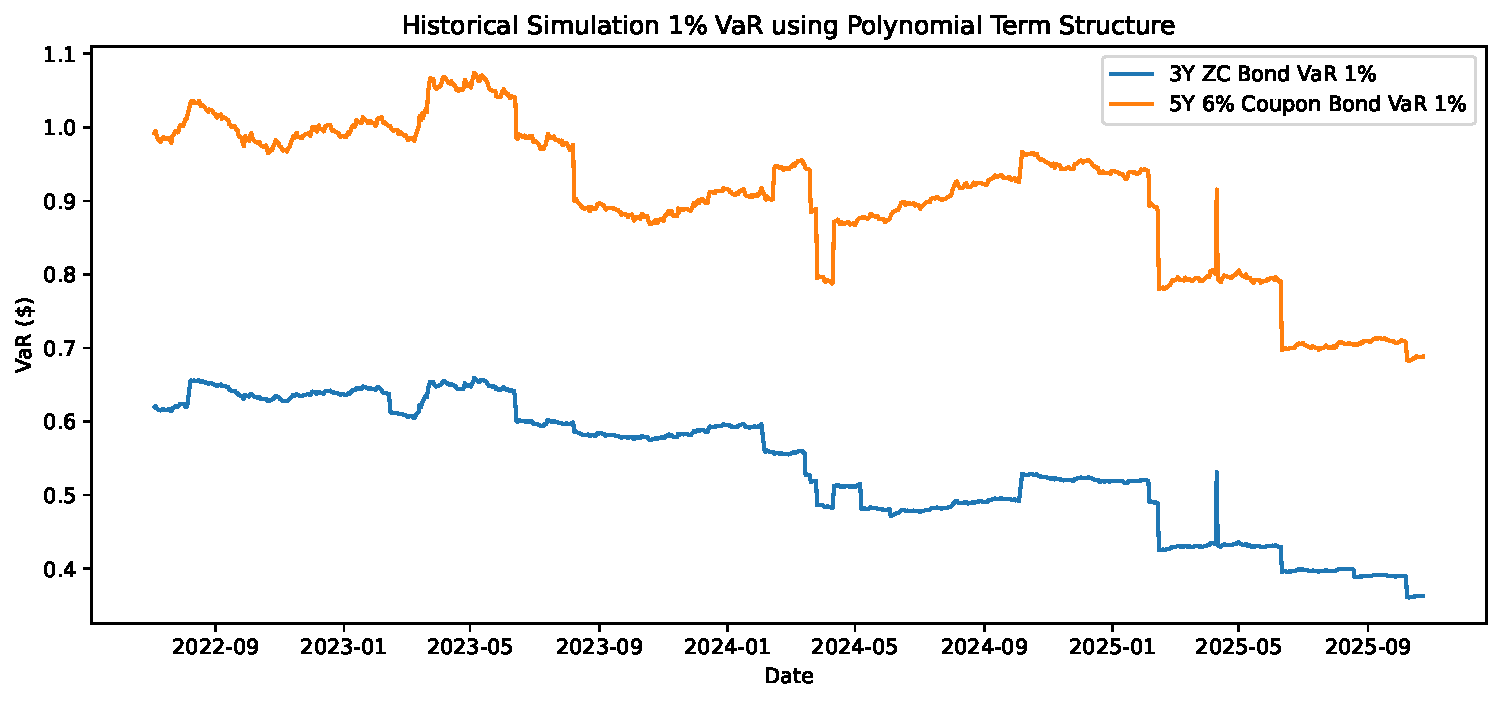
\includegraphics[width=.8\textwidth]{./figures/ECO491_HW4_Q2.3Yv5Y.pdf}
  \caption{$\text{VaR}_{t+1}^{1\%}$ of 3Y Zero-Coupon Bond v. 5Y Semi-Annual 6\% Coupon Bond}
\end{figure}

\begin{figure}[H]
  \centering
  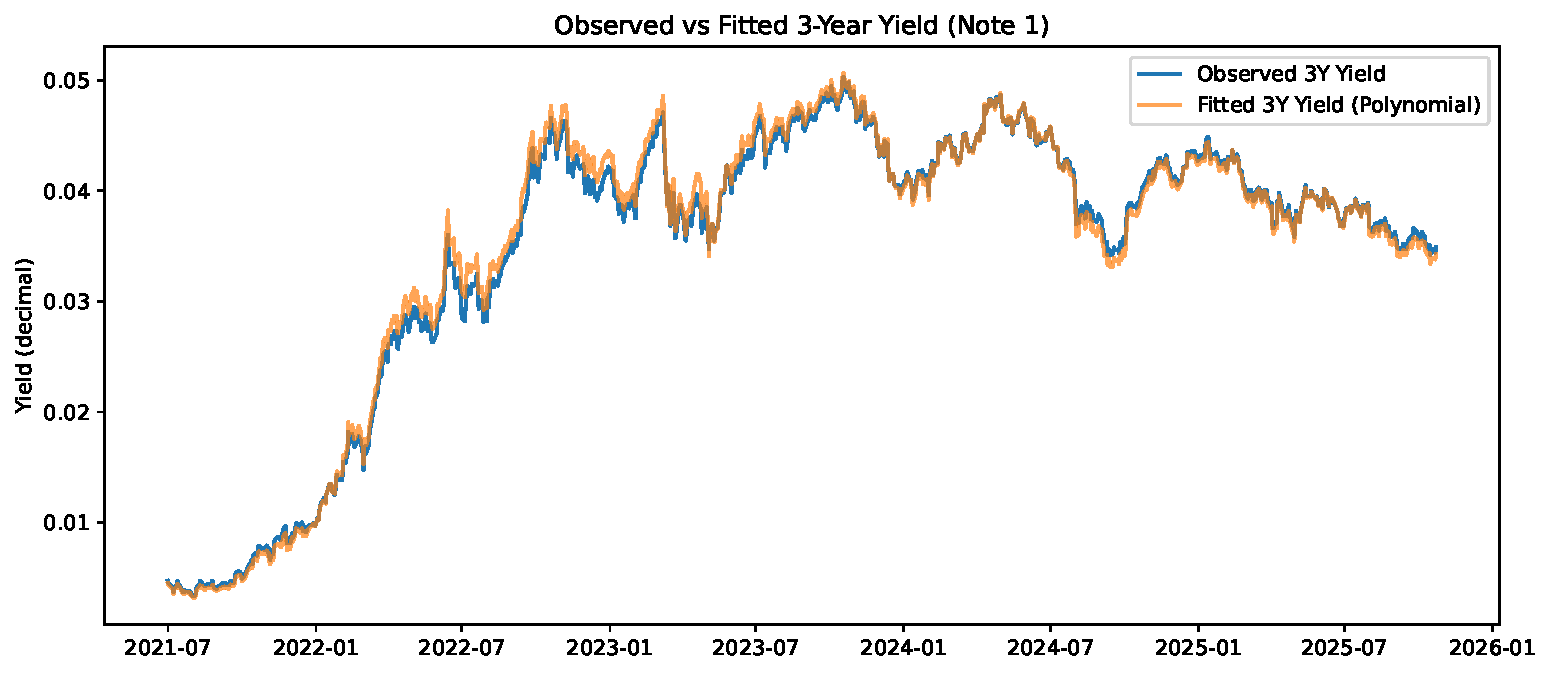
\includegraphics[width=.8\textwidth]{./figures/ECO491_HW4_Q2.Something.pdf}
  \caption{Analytical versus Simulation}
\end{figure}

\section{Nelson–Siegel Model: Analytical Derivation}

The Nelson–Siegel yield curve is given by the following formula:
$$y(\tau) = \beta_{1t} + \beta_{2t} \left( \frac{1 - e^{-\lambda_t \tau}}{\lambda_t \tau} \right)
+ \beta_{3t} \left( \frac{1 - e^{-\lambda_t \tau}}{\lambda_t \tau} - e^{-\lambda_t \tau} \right)$$

The loading associated with the curvature factor is:
\[
C(\tau, \lambda_t) = \frac{1 - e^{-\lambda_t \tau}}{\lambda_t \tau} - e^{-\lambda_t \tau}
\]
\[
\frac{\partial C}{\partial \tau} = -\frac{1 - e^{-\lambda_t \tau}}{\lambda_t \tau^2}
+ \frac{e^{-\lambda_t \tau}}{\tau} + \lambda_t e^{-\lambda_t \tau}
\]
\[
0 = - (1 - e^{-\lambda_t \tau}) + \lambda_t \tau e^{-\lambda_t \tau} + (\lambda_t \tau)^2 e^{-\lambda_t \tau}
\]

Then, let $x = \lambda_t \tau$ to obtain:
$$1 = e^{-x}(1 + x + x^2)$$
$$e^{x} = 1 + x + x^2$$
$$x^* \approx 1.78$$
Hence, the maturity at which the curvature loading reaches its maximum is $\tau^* = \frac{x^*}{\lambda_t} = \frac{1.78}{\lambda_t}$
and the value of the curvature function at its maximum is $C_{\max} = \frac{1 - e^{-1.78}}{1.78} - e^{-1.78} \approx 0.298$, which 
shows that the position of the curvature hump depends inversely on $\lambda_t$, while its height remains constant.

\begin{figure}[H]
  \centering
  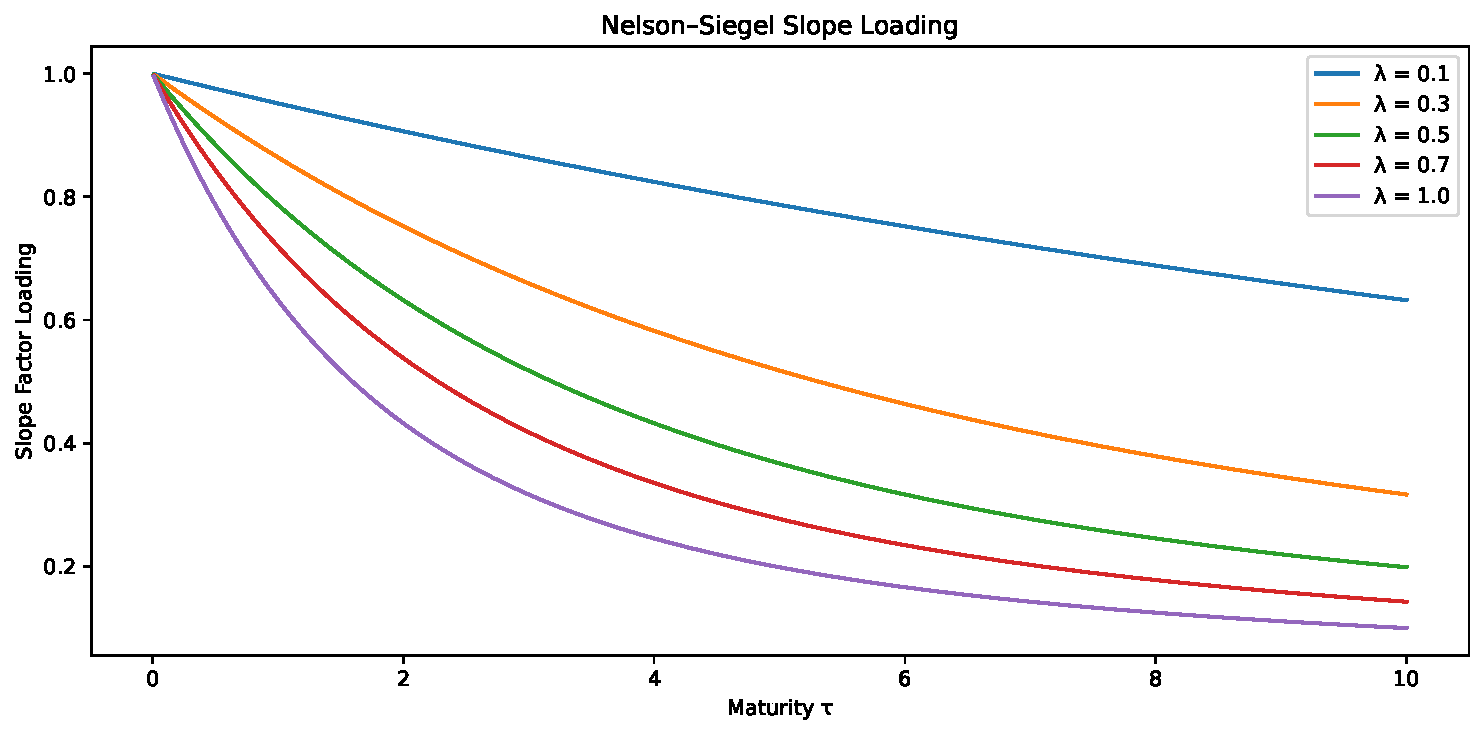
\includegraphics[width=.8\textwidth]{./figures/ECO491_HW4_Q3_Slope.pdf}
  \caption{Slope}
\end{figure}

\begin{figure}[H]
  \centering
  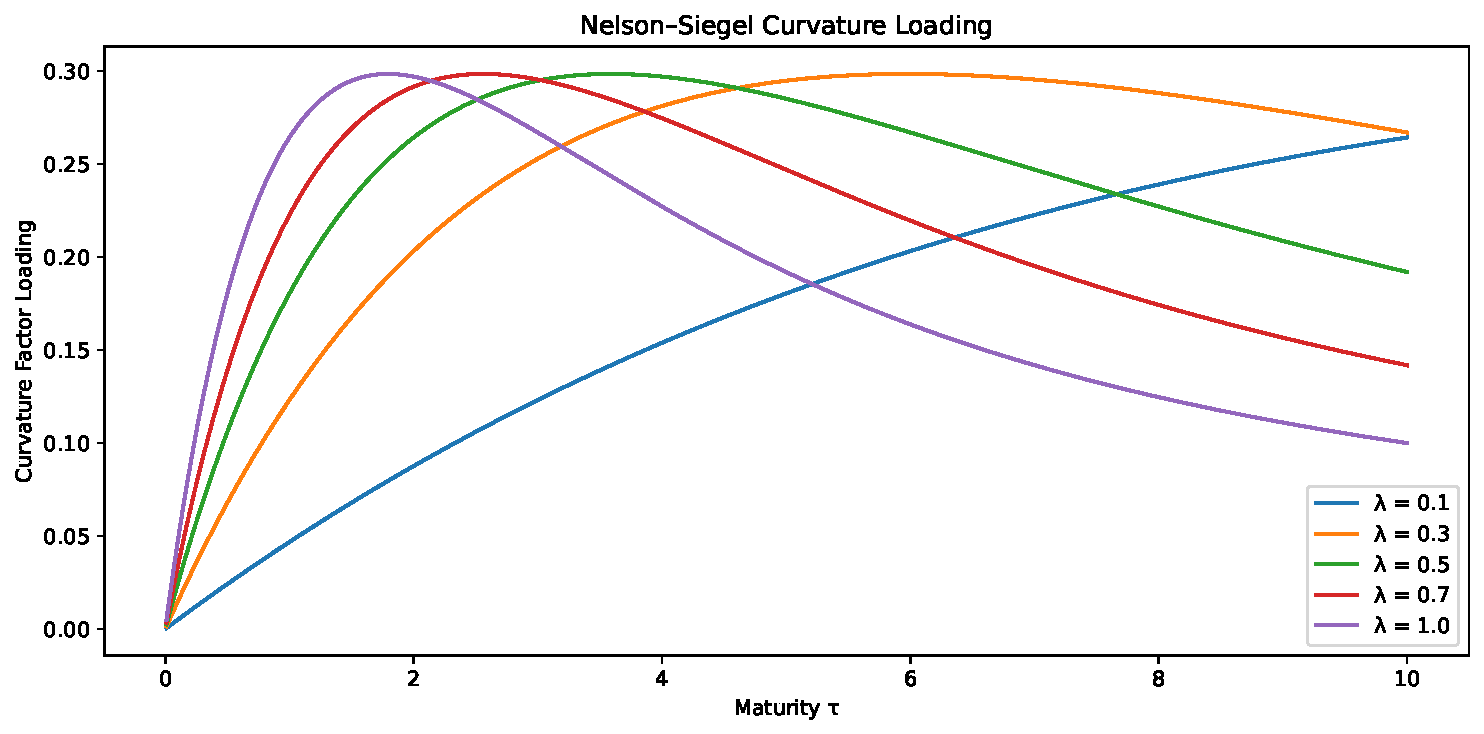
\includegraphics[width=.8\textwidth]{./figures/ECO491_HW4_Q3_Curvature.pdf}
  \caption{Curvature}
\end{figure}

The curvature hump occurs at $\tau = 1.78 / \lambda$. Higher $\lambda$ shifts the hump leftward. Slope loadings are monotonic,
but curvature loadings exhibit the hump structure.